% Created 2017-04-18 Tue 20:26
% Intended LaTeX compiler: pdflatex
\documentclass[11pt]{article}
\usepackage[utf8]{inputenc}
\usepackage[T1]{fontenc}
\usepackage{graphicx}
\usepackage{grffile}
\usepackage{longtable}
\usepackage{wrapfig}
\usepackage{rotating}
\usepackage[normalem]{ulem}
\usepackage{amsmath}
\usepackage{textcomp}
\usepackage{amssymb}
\usepackage{capt-of}
\usepackage{hyperref}
\usepackage{algorithmic}
\author{John Honaker}
\date{\today}
\title{}
\hypersetup{
 pdfauthor={John Honaker},
 pdftitle={},
 pdfkeywords={},
 pdfsubject={},
 pdfcreator={Emacs 25.1.1 (Org mode 9.0.5)}, 
 pdflang={English}}
\begin{document}

\tableofcontents


\section{Variable Selection with Bootstrap in GLM Model for Massive Data}
\label{sec:org50c6091}
\subsection{Summary}
\label{sec:orgc868e23}

Variable Selection with Bag of Little Bootstraps for Generalized Linear Regression

One method for variable selection in a linear regression setting is the LASSO. Traditional linear regression involves finding a solution, \(\beta\), that minimizes \(\| Y - X\beta \|^2_2\). In the LASSO, we trade a small bit of bias, determined by the choice of a regularizatieon hyperparameter, \(\lambda\), to \emph{shrink} the parameters toward zero, and even setting some to zero. The problem is equivalent to minimizing $$ \|Y - X\beta \|^2_2 + \lambda \| \beta \|_1.$$


We can find a solution by applying the Cyclic Coordinate Descent algorithm to the above equation.

   One of the drawbacks of the major drawbacks of t      \hline
he LASSO is the lack of a measure of uncertainty of the estimate, in the sense of how sensitive it is to the obs      \hline
erved data versus the true data generating mechanism. We can asses this variablity by using a bootstrap variable selection procedure. Essentially, we use bootstrap resamples and a model averaging voting scheme similar to random forests. A regression coefficent recieves a vote for each resample that estimates the parameter to be non-zero. The proportion of votes to resamples above a threshold is then used to select variables.

In the context of a massive dataset, the computational cost of even a small number of boostrap resamples becomes very large. However, given that we have a large dataset, we can use only a portion of our data for each replicate. This allows us to drastically reduce the computational cost while still obtaining a good bootstrap estimate.

\section{BLBVS}
\label{sec:org3f594a3}
\subsection{Motivation}
\label{sec:orgfc4c300}
The Bag of Little Bootstraps variable selection method was introduced to give a boostrap variable selection process for massive data sets.

The method should have comparable accuracy to the naive estimator, but hopefully be much faster computationally.
\subsection{Bag of Little Bootstraps}
\label{sec:orga50a4c2}
The algorithm for the BLBVS procedure is as follows. Partition the set of observed data \((x_1, ..., x_n)\) into \(s\) randomly selected subsets (called bags) of size \(b = \{n^\gamma : \gamma \in \(0, 1\) \}\) chosen \emph{without replacement}. Each subset produces \(r\) bootstrap resamples chosen \emph{with replacement} of size \(n\), the original sample size. Notice that each resample can only have at most \(b\) distinct data points.
\subsubsection{Notation}
\label{sec:org005b3cb}
\subsubsection{Algorithm}
\label{sec:org0b7d72c}
\begin{algorithm}
\hline
  \caption{Bag of Little Bootstraps Variable Selection (BLBVS)}
  \hline
  \begin{algorithmic}
    \STATE \textbf{Input:} Original data, $X = (x_1, ..., x_n)$
    \STATE $b:$ size of each subset
    \STATE $s:$ number of subsets
    \STATE $r:$ number of resamples
    \STATE $\beta:$ parameter vector
    \STATE $\xi:$ assessmend of estimator quality
    \STATE \textbf{Output:} An estimate of $\xi$ and the selection result proportion p
    \FOR{$i = 1$ to $s$}
    \STATE Randomly select a subset $\mathcal{I} = \{ i_1, ..., i_b \}$ of $b$ objects from $\{1, 2, ..., n \}$ without replacement
    \STATE Form the subset $\tilde{X}^{(i)}$ based on the original dataset $X$ and index set $\mathcal{I}$
    \FOR{$j = 1$ to $r$}
    \STATE Generate $r$ bootstrap resamples: randomly draw a resample $X^*_{ij} = (\tilde{X}^{(i)}; n^{*ij})$ of size $n$ from subset $\tilde{X}_i$ with replacement, where each resample is $Multinomial(n, (1/b)\mathbf{1}_b)$ distributed with a weight vector of parameters $\beta$ and calculate $\mathbf{1}(\hat{\beta}(X^*_{ij}))$.
    \ENDFOR
    \STATE Get $r$ estimated results of parameter vector $\beta$ and then calculate the standard error a parameter estimation $\xi^{*(i)}$
    \ENDFOR
    \STATE Compute the final estimate of $\xi$ by $s^{-1}\sum^s_{i=1} \xi^{*(i)}_i$
    \RETURN the proportion $p$
    \end{algorithmc}
    \hline
\end{algorithm}

\subsection{BLB Variable Selection}
\label{sec:org5200d53}
\subsubsection{Voting}
\label{sec:org6e0d015}
\subsubsection{Selection}
\label{sec:orgb4c1367}
Let \(\hat{\beta_{ij}}\) be a vetor of estimators for the \(j\text{th}\) resample of the \(i\text{th}\) subset, and \(\hat{\xi}_i\) be the standard error of the parameter estimation in the \(i\text{th}\) subset. The overall standard error \(\hat{\xi}\) is simply the average over the \(\hat{\xi}_i\).

To perform variable selection, we consider indicator functions, \(\mathbf{I} \left( \hat{\beta}_{ijk} \neq 0 \right)}\), to represent whether or not the parameter estimate \(k\) in the \(j\text{th}\) resample of the \(i\text{th}\) subset was set to zero. The selection procedure is based on model averaging using a vote criterion similar to Random Forests. Each bootstrap sample is given an equally weighted vote, for a total of \(s \times r\) votes. A predictor is selected if it recieves a proportion of votes, \(p_k\), greater than some pre-chosen cutoff \(c\). Where \(p_k\) is defined as $$p_k = \frac{\sum^s_{i=1} \sum^r_{j=1} \mathbf{I}(\hat{\beta}_k (X_{ij}) \neq 0)}{s \times r}.$$

\subsection{BLBVS with Group Lasso Penalty for GLM}
\label{sec:orge896770}
\subsubsection{Extending to GLM}
\label{sec:orgdbd3111}
The variable selection method (BLBVS) works perfectly well for a traditional linear regression with continuous predictors. However, it does not handle generalized linear models with categorical predictors or different link functions properly.

For a categorical predictor with \(k\) categories, \(k-1\) dummy variables must be added to the model. Under the original Lasso framework, the dummy variables are penalized individually. This may cause a partial choice of some of levels of the predictor. Ideally, all the dummy variables from a certain category should be chosen or eliminated together. An extension to the Lasso, called the Group Lasso, can overcome these issues by grouping sets of related dummy variables together and penalizing them together. The estimator is defined as $$\hat{\beta}_\lambda = argmin(\| Y - X \beta \|^2_2 + \lambda \sum^G_{g=1} \|\beta I_g \|_2)$$ where \(I_g\) is the index set of the \(g\text{th}\) group of variables, \(g = 1,...,G\) .

To extend the method to a GLM framework, the cost function must be extended to incorporate the link function. The first term of the Lasso cost function then becomes \(\| Y - g^{-1}(X\beta) \|^2_2\) insetad of simply \(\| Y - X\beta \|^2_2\). Consider the following setup of logistic regression for more details. Let \(Y_i\) be a binary response variable, and \(\mathbf{X}\) be the matrix of p independently and idendically distributed predictor variables. The predictor variables are divided into \(G\) groups. Each continuous predictor is its own group with \(df_g = 1\). Each set of dummy variables pertaining to a single categorical variable (with \(k\) levels) is collected as one group with \(df_g = k - 1\). \(\mathbf{X}\) can now be partitioned groupwise by columns so that the linear model becomes $$g(\mathbf{Y}) = log \left( \frac{p_\beta(\mathbf{X})}{1 - p_\beta (\mathbf{X})} \right) = \beta_0 + \sum^G_{g=1} X^T_g \beta_g $$ where \(p_\beta(x) = P_\beta(Y = 1 | x)\) and \(\beta_g \in \mathcal{R}^{df_g}\). This problem is equivalent to minimizing the convex function: $$S_\lambda(\beta) = -l(\beta) + \lambda \sum^G_{g=1} s(df_g) \|\beta_g \|_1$$ where \(l(\cdot)\) is the log-likelihood and \(s(\cdot)\) is chosen to rescale the regularization term with respect to the degrees of freedom in the group. Typically, the value of \(\lambda\) is chosen via cross-validation.

\subsection{Simulations}
\label{sec:org0727da9}
\subsubsection{Setup}
\label{sec:org8f04114}
\subsubsection{Results}
\label{sec:org6723a4b}
\subsubsection{Evaluation}
\label{sec:orgda99d6a}
For the simulation analysis of the BLBVS method, they considered logistic regression with continuous independent predictors as the true model and Group Lasso as the penalty funciton. In this paper, they performed simulations considering \(b = n^\gamma\) with \(\gamma \in \left\{ 0.6, 0.7, 0.8 \right\}\) and let \(r = 100\) in each subset.

The simulated dataset was set to have \(n = 20,000\) and 35 continuous predictors goruped into 8 groups:

\begin{center}
\begin{tabular}{ll}
Index Var & Index Variables\\
\hline
\(\mathcal{I}_1\) & \(\left\{ 1, ..., 5 \right\}\)\\
\(\mathcal{I}_2\) & \(\left\{ 6, ..., 9 \right\}\)\\
\(\mathcal{I}_3\) & \(\left\{ 10, ..., 15 \right\}\)\\
\(\mathcal{I}_4\) & \(\left\{ 16, ..., 20 \right\}\)\\
\(\mathcal{I}_5\) & \(\left\{ 21, ..., 25 \right\}\)\\
\(\mathcal{I}_6\) & \(\left\{ 26, ..., 28 \right\}\)\\
\(\mathcal{I}_7\) & \(\left\{ 29, ..., 31 \right\}\)\\
\(\mathcal{I}_8\) & \(\left\{ 32, ..., 35 \right\}\)\\
\end{tabular}
\end{center}

Coefficients were chosen groupwise to be included in the true model, \(T\), and if \(\mathcal{I}_g \in \mathcal{I}_T\), then the corresponding parameter was given a value of 10. Variables not chosen for the true model, were given random values chosen from a \(N(0, 1)\) distribution. These are intended to be regularized to zero. Simulated \(Y_i\) were drawn from independent Bernoulli distributions where, $$p_\beta(x) = \left[1 + \exp{-\tilde{\mathbf{X}}^T_{i, G} \mathbf{\beta}_G} \right]^{-1}.$$

For the simulations, \(\mathcal{I}_T = \mathcal{I}_{1, 2, 4, 6, 7}\). The figure below shows the selection results for BLBVS with the various values of \(\gamma\) as well as the results for the BootVS without bagging.

\begin{center}
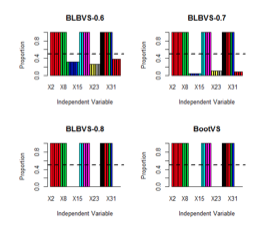
\includegraphics[width=.9\linewidth]{./simresults.png}
\end{center}

The selection results perform equally well under both procedures, even when we set a simple cutoff at being chosen in 50 percent of the replicates. The results show that the proportion estimate becomes more accurate as \(\gamma\), the proportion of the original dataset included in each bagged subset, increases. Logically, the performance of BootVS is superior to BLBVS when \(\gamma\) is small since it resamples from all distinct data points instead of subsets. It has been estimated that each resample in BootVS contains approximately \(0.632n\) different data points in comparison to BootVS's \(n^\gamma\). Thus, it makes sense that the superiority of BootVS decreases as \(\gamma\) increases, and the figure shows that they are effectively equivalent when \(\gamma = 0.8\). Notice however, that BootVS and BLBVS select the correct model.

\subsection{{\bfseries\sffamily TODO} Convergence Properties}
\label{sec:org59a98c9}
\subsubsection{Relative Deviation}
\label{sec:orge287779}


\subsection{{\bfseries\sffamily TODO} Scalability and Computational Analysis}
\label{sec:org14cbaa5}
\subsubsection{Performance of BLBVS}
\label{sec:org4133371}
\subsubsection{Paralellization of Bags}
\label{sec:org4783a46}

\subsection{Real Data Analysis}
\label{sec:org715eb6d}
\subsubsection{Data}
\label{sec:org39d6f79}
Credit card records from Taiwanese bank
\begin{itemize}
\item Goal: Select predictors that important for predicting credit risk
\item Greater than 800 million observations (11 GB)
\item 25 Categorical predictors
\item Binary response (1 - Risky, 0 - Not risky)
\end{itemize}
\subsubsection{Selected Variables}
\label{sec:org23d02f3}
Consistent across methods
\begin{itemize}
\item Force to stop credit card
\item Living Area
\item Education Background
\item Occupation
\item Housing Situation
\item Avg. Monthly Income
\item Family Economic Level
\end{itemize}
\subsubsection{Computational Performance}
\label{sec:orgaeb4c3d}

\begin{center}
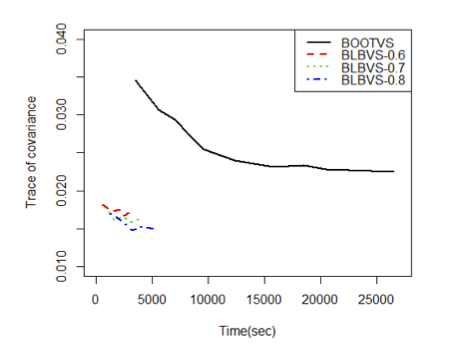
\includegraphics[width=.9\linewidth]{./realresults.png}
\end{center}

\section{Conclusions}
\label{sec:orgf594eff}

\begin{itemize}
\item 
\end{itemize}
\end{document}
